

\chapter{L'esperimento OPERA}

\section{Esperimenti con acceleratori nel dominio di massa indicato dai neutrini atmosferici}

Nel capitolo precedente si \`{e} visto che le attuali evidenze sperimentali per le oscillazioni 
di neutrino vengono da osservazioni fatte con neutrini solari, recentemente confermate 
dall'esperimento Kamland \cite{Kamland} operante con neutrini provenienti da reattori nucleari, e da 
osservazioni fatte con neutrini atmosferici. L'eccesso di eventi indotti da $\overline{\nu }_{e}$ rilevato
dall'esperimento LSND \cite{A32} e imputabile a oscillazioni di neutrino resta non confermato da altri
esperimenti.

Nel caso dei neutrini atmosferici, i risultati sperimentali conducono
a suggerire l'esistenza di oscillazioni $\nu _{\mu }\rightarrow \nu
_{\tau }$ nella regione dei parametri corrispondente a $\Delta m^{2} =
( 1.5\div 3.4) \times 10^{-3}$ $eV^{2}$ e $\sin ^{2}2\theta \sim
1$. Vengono invece sfavoriti il canale $\nu _{\mu }\rightarrow \nu
_{e}$ e l'oscillazione di $\nu _{\mu } $ in neutrini sterili, cio\`{e}
non visibili tramite le interazioni deboli.

Per esplorare con fasci prodotti da acceleratori di particelle il suddetto dominio dei parametri 
di oscillazione, con valori
di $\Delta m^{2}$ cos\`{i} bassi, sono necessari esperimenti con un rapporto $\frac{L}{E%
}$ che si approssimi a quello dei neutrini atmosferici, ove $L$ \`{e} la distanza tra
sorgente e rivelatore ed $E$ \`{e} l'energia del fascio, e quindi con un distanza sorgente-rivelatore 
relativamente alta. Sono questi i cosiddetti esperimenti a \emph{long baseline} (LBL). 

E' possibile dimostrare, infatti, che in presenza di fondo la sensibilit\`{a} in $\Delta
m^{2}$ di un esperimento di apparizione migliora con la radice quadrata di $L$. 
\`{E} solo nel caso ideale di assenza di fondo che essa risulta
indipendente da $L$, migliorando con la radice quadrata
della massa del rivelatore e con l'inverso dell'energia. In generale, gli esperimenti su long baseline, 
traggono notevole vantaggio dalla grande distanza del rivelatore dalla sorgente del fascio, che riduce
drasticamente il numero di eventi di fondo.

La figura 2.1 mostra le regioni del piano $\sin ^{2}2\theta -\Delta m^{2}$
esplorabili con esperimenti a LBL e con esperimenti a {\emph{short baseline}} (SBL).

\begin{figure}[tbp]
\begin{center}
\includegraphics[width=80mm,height=95mm]{./figure_cap2/figura2_1.eps}
\end{center}
\caption{Regioni esplorabili con esperimenti LBL e SBL.}
\end{figure}

 Uno dei principali ostacoli alla realizzazione di 
esperimenti a LBL \`{e} indotto dalla naturale divergenza del fascio, che
riduce fortemente il flusso di neutrini che giungono al rivelatore. Il
flusso emesso da una sorgente, infatti, pu\`{o} essere scritto come:

\begin{equation}
\Phi =\frac{dN_{\nu }}{dA}  \tag{2.1}
\end{equation}
dove $dN_{\nu }$ indica il numero di neutrini che, nell'unit\`{a} di tempo,
attraversano una superficie di area $dA$ disposta perpendicolarmente al fascio. Per
un angolo solido $d\Omega $ si ha:

\begin{equation}
dA=L^{2}\cdot d\Omega  \tag{2.2}
\end{equation}
che, unita alla (2.1), fornisce:

\begin{equation*}
\Phi \propto \frac{1}{L^{2}}
\end{equation*}
Il flusso risulta quindi inversamente proporzionale al quadrato della
distanza.

Ad esempio, in un esperimento LBL con $L\simeq 10^{3}$ $Km$ il flusso
di neutrini che giunge al rivelatore risulta circa un milione di volte
pi\`{u} basso di quello in un esperimento con $\% L\simeq 1$ $Km$ che
utilizzi lo stesso rivelatore sulla stessa linea del fascio.  Di
conseguenza, se con un esperimento SBL si prevede di rivelare, in un
certo periodo di tempo, un numero di eventi di corrente carica $\nu_\mu$ 
dell'ordine di $10^{6}$, in un esperimento LBL, operante con lo
stesso bersaglio e sulla medesima linea di fascio, si otterr\`{a} un
solo evento. Ci\`{o} significa, inoltre, che se la massa del
rivelatore SBL \`{e} dell'ordine di $1$ $ton$ (come in CHORUS e
NOMAD), per un esperimento LBL con un bersaglio di massa $\sim 1$
$kton$ si ha un numero di eventi inferiore di circa tre ordini di
grandezza.

Gli obbiettivi della prossima generazione di esperimenti volti ad
approfondire mediante l'uso di fasci prodotti da acceleratori lo
studio degli effetti osservati con neutrini atmosferici sono
l'osservazione diretta di oscillazioni $\nu_\mu \rightarrow \nu_\tau$
tramite apparizione di $\nu_\tau$ e una misura piu' precisa dei
parametri di oscillazione.  Nei limiti della sensibilita' degli
esperimenti, verra' inoltre ricercata la presenza di oscillazioni
"sub-dominanti" $\nu_\mu \rightarrow \nu_e$.

Negli Stati Uniti il progetto \textbf{NuMI} \cite{B1} prevede l'invio
dei neutrini muonici dal Fermilab (FNAL) alla miniera Soudan nel
Minnesota (posta ad una distanza di $730$ $Km$) in cui \`{e} situato
il rivelatore MINOS \cite{B2}. Questo rivelatore e' essenzialmente uno
spettrometro per muoni, costituito da lastre di ferro magnetizzato per
una massa di $5.4$ $kton$. Si tratta di un esperimento di sparizione
di $\nu _{\mu }$, dunque l'oscillazione $% \nu _{\mu }\rightarrow \nu
_{\tau }$ puo' venire misurata soltanto in termini di eccesso
statistico di eventi senza muone nello stato finale. L'apparato
sperimentale e' inoltre in grado di osservare eventi con elettrone
nello stato finale, pur non essendo ottimizzato per questo
scopo. Verra' quindi eseguita anche una ricerca di oscillazioni
$\nu_\mu\rightarrow \nu_e$. La presa dati sta ora iniziando.

In Europa, un progetto congiunto CERN - INFN prevede l'invio del fascio di
neutrini muonici del fascio CNGS \cite{B3} dal CERN ai Laboratori Nazionali del Gran
Sasso, posto ad un distanza $L\simeq 732$ $Km$. L'energia media del fascio (%
$E_{\nu }\simeq 17.7$ $GeV$) \`{e} ottimizzata per lo studio di apparizione $%
\nu _{\mu }\rightarrow \nu _{\tau }$. La ricerca di oscillazioni
 $\nu _{\mu }\rightarrow \nu _{\tau }$, basata
sulla ricerca diretta dell'apparizione, necessita infatti di fasci di $\nu _{\mu }$ dotati
di energia superiore alla soglia di produzione del leptone $\tau $ (ossia $%
E_{\nu }>3.6$ $GeV$).

Come per gli esperimenti SBL, sono possibili due approcci per la
rivelazione del $\tau $:

\begin{itemize}
\item  sfruttare esclusivamente le caratteristiche cinematiche peculiari del decadimento
del $\tau $;
\item  identificare il $\tau $ attraverso l'osservazione diretta del suo
decadimento e ricorrere allo studio della cinematica del decadimento solo per una
ulteriore riduzione del fondo.
\end{itemize}

Sul primo tipo di approccio si basa l'esperimento \textbf{ICARUS} \cite{B4},
il cui rivelatore si compone di quattro moduli, ciascuno dei quali \`{e}
costituito da una Time Projection Chamber (TPC) ad Argon liquido.

Il secondo approccio \`{e} quello seguito dall'esperimento \textbf{%
OPERA} \cite{B5}, al quale \`{e} dedicato il presente capitolo.

Ambedue gli esperimenti sono anche in grado di osservare eventi con un elettrone
nello stato finale e quindi di ricercare oscillazioni $\nu_\mu\rightarrow \nu_e$.

Il fascio CNGS verra' operato a partire da meta' del 2006.

\section{Il fascio CNGS}\label{sec:cngs}

Il fascio di neutrini \textbf{CNGS} (\textbf{C}\emph{ERN} \textbf{N}\emph{%
eutrino} \emph{to} \textbf{G}\emph{ran} \textbf{S}\emph{asso}) sar\`{a}
prodotto dal \textbf{SPS} (\textbf{S}\emph{uper} \textbf{P}\emph{roto} 
\textbf{S}\emph{incrotrone}) del CERN facendo interagire protoni accelerati un'energia
 di $400$ $GeV$ su un bersaglio costituito da 13 cilindri di carbonio di $10$ $cm$ di
lunghezza e $4$ $cm$ di diametro. I mesoni $\pi ^{+}$ e $K^{+}$ che ne
derivano saranno collimati lungo la direzione di volo verso il Gran Sasso,
mediante un sistema costituito da due lenti di focalizzazione e decadono
all'interno di un tunnel lungo $1$ $Km$. Alla fine del tunnel \`{e} posto  un %
\emph{hadron stop}, che ha il compito di assorbire i protoni che non hanno
interagito col bersaglio ed i mesoni che non sono decaduti entro il tunnel.
Esso \`{e} realizzato con un blocco, lungo $18$ $m$, di grafite e di ferro.
Per controllare il fascio di neutrini, saranno utilizzate due stazioni di
rivelatori al silicio, una posta subito dietro l'hadron stop, l'altra
separata da 67 metri di roccia.

La tabella 2.1 riporta le caratteristiche nominali del fascio. In figura
2.2 \`{e} mostrato lo schema della linea del fascio ed in figura 2.3 lo
spettro energetico dei neutrini $\nu _{\mu }$ attesi al Gran Sasso.

\begin{table}[tbp]
\begin{center}
\begin{tabular}{||c|c||}
\hline\hline
$\nu _{\mu }[m^{2}$ $pot]$ & $7.78\times 10^{-9}$ \\ \hline
$E_{\nu _{\mu }}[Gev]$ & $17.7$ \\ \hline
$\nu _{\mu }CC[eventi/pot/kt]$ & $5.85\times 10^{-17}$ \\ \hline
$\overline{\nu }_{\mu }/\nu _{\mu }$ & $2.1\%$ \\ \hline
$\nu _{e}/\nu _{\mu }$ & $0.8\%$ \\ \hline
$\overline{\nu }_{e}/\nu _{\mu }$ & $0.07\%$ \\ \hline
$\nu _{\tau }$ & \textbf{trascurabile} \\ \hline\hline
\end{tabular}
\end{center}
\caption{Caratteristiche nominali del fascio CNGS.}
\end{table}

\begin{figure}[tbp]
\begin{center}
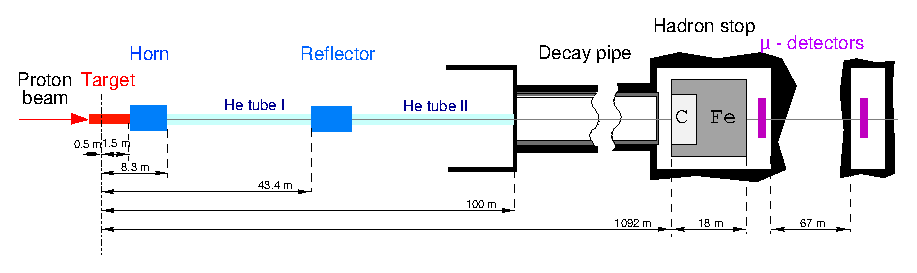
\includegraphics[width=130mm,height=40mm]{./figure_cap2/figura2_2.eps}
\end{center}
\caption[Struttura del fascio CNGS.]{Configurazione della linea di fascio CNGS}
\end{figure}

\begin{figure}[tbp]
\begin{center}
\includegraphics[width=80mm,height=75mm]{./figure_cap2/figura2_3.sh}
\end{center}
\caption{Spettro in energia del fascio di $\protect\nu _{\protect\mu }$ del
CNGS atteso al Gran Sasso.}
\end{figure}

Assumendo 200 giorni di funzionamento all'anno, il numero di \emph{pot}
(protoni su bersaglio) attesi operando il fascio assieme al collisionatore protone-protone
 LHC \`{e} pari a $4.5\times 10^{19}/anno$.

Il numero di interazioni da neutrino, includendo tutti i sapori e
considerando anche gli eventi di corrente neutra, \`{e} pari a $\sim 35000$%
, per un rivelatore di massa $1.8$ $kt$ e 5 anni di esposizione al fascio.
Il corrispondente numero di interazioni di corrente carica di $\nu _{\tau }$ \`{e}
pari a circa 130, per $\Delta m^{2}=2.4\times 10^{-3}$ $eV^{2}$ e mescolamento massimo
(ossia $\sin ^{2}2\theta =1$). Appare possibile che l'intensita' del fascio sia aumentata di un
fattore $1.5$ rispetto a quella nominale prevista nel progetto iniziale, a cui si riferiscono 
i suddetti numeri di interazioni.

\section{L'esperimento OPERA}

\textbf{OPERA} (\textbf{O}\emph{scillation} \textbf{P}\emph{roject with} 
\textbf{E}\emph{mulsion t}\textbf{R}\emph{acking} \textbf{A}\emph{pparatus})
\`{e} un esperimento per l'osservazione di oscillazioni $\nu _{\mu }\rightarrow \nu _{\tau }$
su \emph{ long baseline} nel
fascio CNGS, tramite la rivelazione dell'apparizione del $\nu
_{\tau }$ attraverso l'osservazione della produzione
del leptone $\tau $ (figura 2.4). La ricerca dell'apparizione del $\nu
_{\tau }$ viene effettuata nella regione
dei parametri indicata dalle osservazioni con muonici atmosferici. Il rivelatore e' posto
nei laboratori sotterranei del Gran Sasso, a circa $730$ $Km$ di distanza
dal CERN.
L'esperimento � sensibile anche alle oscillazioni di  $\nu_\mu \rightarrow\nu_e$,
in una regione di parametri di oscillazione pi� estesa rispetto agli esperimenti condotti
sino ad ora.

\begin{figure}[tbp]
\begin{center}
\includegraphics[width=130mm,height=40mm]{./figure_cap2/figura2_5.eps}
\end{center}
\caption{Schema delle oscillazioni dei neutrini provenienti dal CERN.}
\end{figure}

La rivelazione del $\nu _{\tau }$ consente di identificare l'avvenuta
oscillazione $\nu _{\mu }\rightarrow \nu _{\tau }$, in quanto il fascio
proveniente dal CERN non contiene neutrini in misura apprezzabile  $\nu _{\tau }$.
Anche pochi eventi di segnale possono essere sufficienti a dimostrare
l'ipotesi di oscillazione, purch\'{e} il fondo venga mantenuto sempre ad un
basso livello.

In OPERA, lo strumento di base per la reiezione del fondo e' l'osservazione del decadimento del tau.
Il leptone tau ha una vita media breve ($c\tau \sim 87$ $\mu m$). In base alla
distribuzione in energia del fascio CNGS, si ottiene la distribuzione delle
lunghezze di decadimento del $\tau $ riportata in figura 2.5. Alle energie del CNGS,
 il leptone $\tau $ decade in media dopo circa $0.5 mm$. Per osservare sia la produzione che 
il decadimento del
leptone tau occorre quindi utilizzare una tecnica che offra altissime 
granularita' e risoluzione spaziale. Le tecnica delle \emph{ emulsioni nucleari}
presenta caratteristiche uniche
 sotto questo aspetto. Dopo lo sviluppo, i "grani" delle emulsioni hanno dimensioni dell'ordine
 del micron e permettono di ottenere risoluzioni sub-micrometriche.
 
L'utilizzo di emulsioni nucleari ha importantissimi precedenti nella
fisica delle particelle elementari, in particolare per l'osservazione
di particelle a vita breve.  Fu lo sviluppo di questa tecnica che
permise nel 1947 la scoperta del pione attraverso il suo decadimento
in muone nell'esperimento Lattes-Occhialini-Powell \cite{pione}. La
prima osservazione delle particelle poi definite come "charmate" dopo
la loro chiarissima osservazione al BNL e a SLAC \cite{jpsi1,jpsi2,jpsi3}
avvenne nel 1971 in un esperimento con raggi cosmici in cui erano
utilizzate emulsioni nucleari \cite{Niu}. L'esperimento WA75 at CERN
effetuo' la prima osservazione diretta del decadimento di una
particella dotata di "beauty" \cite{beauty}

\begin{figure}[tbp]
\begin{center}
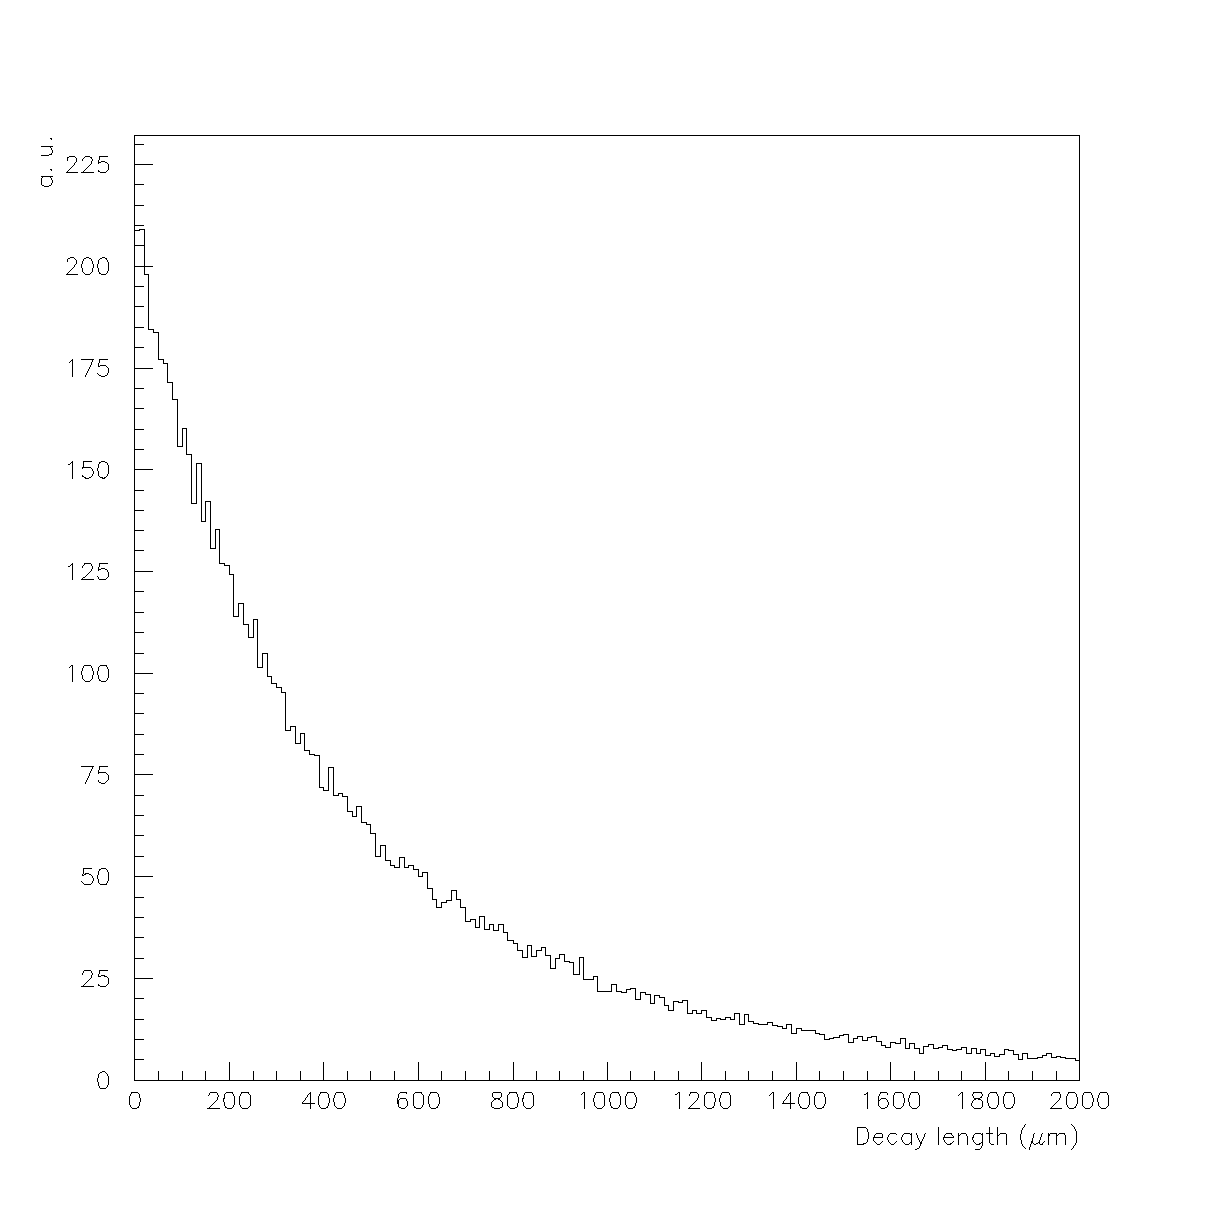
\includegraphics[width=95mm,height=95mm]{./figure_cap2/decadim_tau_CNGS.eps}
\end{center}
\caption{Distribuzione delle lunghezze di decadimento del $\protect\tau $
prevista nell'esperimento OPERA.}
\end{figure}
 
La struttura del rilevatore � stata quindi pensata allo scopo di
identificare la traccia del leptone $\tau$ e i due vertici che segnano
la sua produzione e il suo decadimento: il primario e un secondario
corrispondente al decadimento di tale particella, mediante l'uso di
emulsioni nucleari. Al contempo, data l'esiguita' del flusso di
neutrini a grande distanza dalla sorgente, il rivelatore deve avere
una grande massa, dell'ordine di grandezza delle migliaia di
tonnellate.  Viene quindi fatto ricorso alla tecnica della Emulsion
Cloud Chamber (ECC), introdotta nel 1952 \cite{ECC} . Essa fu
successivamente sviluppata soprattutto in Giappone e utilizzata in
vari esperimenti. Di particolare rilevanza per la ricerca di
oscillazioni $\nu_\mu \rightarrow \nu_\tau$ e' la sua utilizzazione
per l'osservazione di neutrini tau da parte dell'esperimento DONUT
\cite{Donut}.

La tecnica ECC e' basata sull'uso delle emulsioni nucleari per il
tracciamento ad altissima risoluzione spaziale, mentre la massa del
rivelatore viene essenzialmente fornita da lastre di materiale passivo
inframmezzate ai fogli di emulsione nucleare. L'esperimento OPERA
utilizza un bersaglio segmentato, costituito da lastre di piombo
spesse 1 mm (che funge da materiale passivo) alternate a fogli di
emulsioni nucleari. Tale struttura consente la rivelazione diretta del
decadimento del $\tau $, prodotto nella interazione di corrente carica
(CC) dei $\nu _{\tau }$ nel bersaglio :
\begin{equation}
\nu _{\tau }N\rightarrow \tau ^{-}X  \tag{2.3}
\end{equation}

Le interazioni di CC del $\nu _{\tau }$ vengono cosi' identificate
dalla rivelazione del leptone $\tau $ tramite l'osservazione delle sue tipologie di
decadimento e, in particolare, in quelle a singola traccia carica (\emph{single-prong}) 
ossia in un elettrone, un muone o un adrone:
\begin{eqnarray*}
\tau ^{-} &\rightarrow &e^{-}\nu _{\tau }\overline{\nu }_{e} \\
\tau ^{-} &\rightarrow &\mu ^{-}\nu _{\tau }\overline{\nu }_{\mu } \\
\tau ^{-} &\rightarrow &h^{-}\nu _{\tau }(n\pi ^{0})
\end{eqnarray*}

I rapporti di decadimento sono: $17.8\%$ per il canale elettronico, $%
17.4\%$ per il canale muonico e $49.5\%$ per quello adronico con singolo
adrone carico.
Il restante 15.2\% si riferisce al decadimento a tripla traccia carica (%
\emph{multi-prong}): $\tau ^{-}\rightarrow \pi ^{+}\pi ^{-}\pi ^{-}\nu
_{\tau }(n\pi ^{0})$.

I decadimenti a singola traccia carica sono caratterizzati da una configurazione a
 \emph{gomito}, ove la traccia del $\tau $ stesso e quella del suo prodotto di decadimento
carico formano un angolo comunenemente detto \emph{angolo di kink}, come mostrato in figura 2.6.
 La identificazione  dell'evento, in base all'angolo di kink, avviene
grazie all'altissima risoluzione delle emulsioni nucleari.

\begin{figure}[tbp]
\begin{center}
 \includegraphics[height=6cm,width=8cm,angle=270]{./figure_cap2/figura2_4.eps}
\end{center}
\caption{Interazione di corrente carica del $\protect\nu _{\protect\tau }$ con
il successivo tipico decadimento a gomito del $\protect\tau $ in una singola particella carica}.
\end{figure}

L'area totale di emulsioni necessarie necessaria per OPERA \`{e} elevatissima, dell'ordine
 di $\sim 10^{5}$ $m^{2}$. La realizzazione dell'esperimento \`{e} quindi strettamente legata 
allo sviluppo di tecniche di produzione industriale su larga scala di emulsioni nucleari. 
Essa dipende anche strettamente dallo straordinario progresso delle tecniche di 
scansione automatica che sta avendo luogo in questi anni.

La presa dati di OPERA avr\`{a} inizio nel 2006


\section{L'apparato sperimentale}
\subsection{La cella ECC}

Il rivelatore utilizzato dall'esperimento OPERA \cite{B6} presenta una struttura
altamente modulare. Una cella della struttura a ECC \`{e} costituita da una 
lastra di materiale passivo
seguita da un sottile foglio di emulsione nucleare (\emph{ES}, \emph{%
Emulsion Sheet}). Nel caso di OPERA, la lastra di materiale passivo \`{e} una
lamina di piombo spessa $1$ $mm$, mentre il foglio di emulsione \`{e}
ottenuto fissando $\sim 45$ $\mu m$ di gel su entrambe le facce di un
supporto di plastica (\emph{base}) spesso $\sim 200$ $\mu m$ (figura 2.7).

L'alta densit\`{a} del piombo permette di ottenere un rivelatore di grande massa con
una minima distanza tra i fogli di emulsione. Vengono cos\`{i} minimizzati i decadimenti del 
$\protect\tau$ nella stessa lastra di materiale passivo in cui esso \`{e} prodotto, pi\`{u}
difficili da identificare. Inoltre l'alto Z e quindi la bassa lunghezza di radiazione del piombo
(Xo = 5,6 mm)  consentono la misura della quantit\`{a} di moto per diffusione multipla coulombiana, 
nonch\'{e} l'identificazione degli elettroni e la misura della loro energia
tramite l'osservazione degli sciami elettromagnetici da essi generati. La
radioattivit\`{a} naturale residua del piombo va tuttavia tenuta sotto controllo, al fine di 
evitare che le emulsioni vengano impressionate da tracce di fondo
(\emph{background}).

\begin{figure}[tbp]
\begin{center}
\includegraphics[width=110mm,height=60mm]{./figure_cap2/figura2_6.eps}
\end{center}
\caption[Struttura schematica di una cella ECC.]{Struttura schematica di una
cella ECC; nel caso, rappresentato in figura, in cui il $\protect\tau $ decade a valle della
 lastra di piombo in cui 
\`{e} stato prodotto, l'angolo di kink viene ricostruito tramite i quattro segmenti di
traccia nei films di emulsione.}
\end{figure}

Le emulsioni sono costituite da bromuro di argento immerso in una gelatina. Una volta che esse 
sono sviluppate, il passaggio di una particella carica \`{e} indicato da una serie di \emph{grani}
 di colore scuro. Le emulsioni nucleari sono caratterizzate da una sensibilit\`{a} a \emph{singole}
particelle e dalle costanti e piccole dimensione dei grani, dell'ordine del micron, in modo tale da 
assicurare una elevata risoluzione spaziale.

Il numero di grani anneriti che si formano in $\sim 45$ $\mu m$ di emulsione
 \`{e} dell'ordine di 15 e quindi sufficiente per la ricostruzione di
 \emph{micro-tracce}, anche mediante tecniche di \emph{scansione automatica}.

Il passaggio di una particella carica attraverso una cella ECC genera quindi
un segmento di traccia, o micro-traccia, in ciascuno degli strati di emulsione
da una parte e dall'altra della base di plastica. Connettendo i grani che nelle
due micro-tracce sono prossimi alla base, si ottiene una \emph{traccia di base}. Essa
 consente di ricostruire la traccia della particella con una migliore risoluzione angolare 
(dell'ordine di qualche milliradiante o ancora meglio in caso di misure di precisione)
dato che i grani prossimi alla base di plastica non sono affetti dalle, seppur piccole, 
distorsioni negli strati di emulsione indotte dal processo di sviluppo.

Nel 40\% dei casi, il $\tau $ decade nelle emulsioni o all'interno della
lastra di piombo immediatamente a valle rispetto a quella in cui \`{e}
avvenuta l'interazione primaria del $\nu _{\tau }$; si parla, allora, di 
\emph{decadimento lungo}. Nel restante 60\% dei casi, invece, esso decade entro la
stessa lastra del vertice di interazione (\emph{decadimento corto}).

Nel primo caso, il $\tau $ viene rivelato misurando l'angolo di kink formato
dalla direzione\ della traccia di base lasciata dal $\tau $ stesso e dalla
direzione della traccia di base generata dalla particella prodotta nel
decadimento (figura 2.7). La traccia del $\tau $ si trova nel foglio
d'emulsione che precede la lastra di piombo in cui si \`{e} verificato il
decadimento, mentre la traccia della particella prodotta \`{e} individuata
nel foglio immediatamente sucessivo.

Per i decadimenti corti si adotta, invece, il metodo del \emph{parametro di
impatto} (\emph{IP}). Si localizza anzitutto il vertice di interazione, mediante almeno due tracce.
Un evento \`{e} considerato \emph{candidato} se un'altra traccia, estrapolata all'indietro, ha 
una minima distanza dal vertice, ossia parametro di impatto, superiore ad un valore di soglia 
dipendente dalla posizione longitudinale del vertice ricostruito. Questi eventi presentano un
 rapporto segnale/rumore meno favorevole rispetto a quelli in cui il $\tau $ subisce
un decadimento lungo.

\subsection{La struttura del rivelatore}

In figura 2.8 \`{e} riportata la struttura modulare dell'apparato
sperimentale nella sua attuale configurazione. L'unit\`{a} fondamentale
della struttura \`{e} detta \emph{mattone} (o \emph{brick}) ed \`{e}
costituita da una sequenza in cui lastre di piombo si alternano a fogli di
emulsione, per un totale di 56 celle ECC. L'uso di mattoni consente di
costruire un \emph{bersaglio attivo} altamente modulare e sufficientemente compatto,
con una massa complessiva di $\sim 1.8$ $kt$.

\begin{figure}[tbp]
\begin{center}
\includegraphics{./figure_cap2/figura2_7.eps}
\end{center}
\caption[Schema del rivelatore di OPERA nella sua attuale configurazione.]{%
Schema del rivelatore di OPERA nella sua attuale configurazione. Sono
visibili i moduli del bersaglio e la loro struttura di supporto, 
 fissata alla parte superiore dei due spettrometri per muoni a ferro magnetizzato.}
\end{figure}

Ciascun mattone presenta dimensioni trasverse pari a $(10.2\times 12.7)$ $%
cm^{2}$ che sono frutto di una scelta di compromesso. Una volta avvenuta
l'interazione, infatti, il mattone viene rimosso e le emulsioni vengono
analizzate; la massa del singolo mattone deve garantire la possibilit\`{a} di
poterlo rimuovere con la minima perdita di massa del rivelatore.
Inoltre, l'estrazione di mattoni aventi piccole dimensioni risulta
meccanicamente pi\`{u} semplice.
 D'altra parte, mattoni di dimensioni eccessivamente piccole accentuano
gli effetti di bordo. In tabella 2.2 sono riportate le principali
caratteristiche di un mattone.

\begin{table}[tbp]
\centering
\begin{tabular}{||c|c||}
\hline\hline
Spessore singola cella ECC ($mm$) & $1.3$ \\ \hline
Numero di celle/mattone & $56$ \\ \hline
Numero di fogli di emulsione/mattone & $58$ \\ \hline
Dimensioni trasversali ($cm^{2}$) & $10.2\times 12.7$ \\ \hline
Dimensioni longitudinali ($cm$) & $7.5$ \\ \hline
Dimensioni longitudinali ($X_{0}$) & $10$ \\ \hline
Peso ($Kg$) & $7.9(Pb)+0.4(emulsioni)$ \\ \hline\hline
\end{tabular}
\caption{Caratteristiche di un mattone.}
\end{table}

Grazie alla sua struttura e alle sue dimensioni (figura 2.9), il mattone permette di misurare la 
quantit\`{a} di moto delle particelle tramite la diffusione multipla coulombiana e di
discriminare elettroni da adroni mediante la rivelazione dello sciame
elettromagnetico prodotto nell'attraversamento delle lastre di piombo. Dato il loro grande numero,
i mattoni verranno costruiti da una macchina automatica specialmente progettata,
 detta \emph{Brick Assembly Machine} (BAM).

\begin{figure}[tbp]
\begin{center}
\includegraphics[width=100mm,height=80mm]{./figure_cap2/brick.eps}
\end{center}
\caption{Struttura schematica di un mattone di OPERA.}
\end{figure}

I mattoni sono assemblati in maniera da formare \emph{muri} (o \emph{walls})
verticali da 3328 mattoni (52 in orizzontale $\times $ 64 in verticale), ortogonali alla direzione
del fascio. Le dimensioni complessive di un muro sono $6.7\times 6.7$ $m^{2}$ e la sua massa \`{e}
 $27$ $ton$. La struttura di supporto di un muro (figura
2.10) consta di bande verticali e guide orizzontali sui quali i mattoni
sono posizionati entro una precisione di $1$ $mm$. Essa \`{e} estremamente
leggera ($\sim 0.4\%$ della massa complessiva del bersaglio), essendo stata
progettata con l'obiettivo di minimizzare il numero di interazioni da
neutrino che avvengono in essa e non nei mattoni. Il caricamento dei mattoni nella
struttura in fase di installazione dell'esperimento e la loro estrazione in seguito
a interazioni di neutrini  vengono attuati
tramite un sistema automatico denominato \emph{Brick Manipulator System} (BMS).

\begin{figure}[tbp]
\begin{center}
\includegraphics[width=80mm,height=95mm]{./figure_cap2/figura2_8.eps}
\end{center}
\caption{Struttura di supporto per un muro del rivelatore di OPERA.}
\end{figure}
Ogni muro di mattoni � seguito da due piani di tracciamento elettronici (\emph{Target
Trackers}, \emph{TT}). Questi piani sono realizzati 
mediante \emph{strips} di scintillatore plastico ($2.6$ $cm\times 1$ $cm\times 6.7$ $m$) e
 contengono ciascuno 256 strips. Ogni gruppo di 64 strips costituisce una unit� indipendente 
letta mediante un fotorivelatore a 64-pixels, cosicch\`{e} ogni piano viene letto 
da 8 fotorivelatori. Le strips del \emph{TT} sono larghe 2.6 $cm$ e spesse 1 $cm$.
Vengono abbinati due piani di TT con strips orientate lungo X e rispettivamente lungo Y. Simulazioni 
Monte Carlo hanno confermato che la segmentazione adottata non abbassa eccessivamente
 l'efficienza per l'identificazione del mattone in cui \`{e} avvenuta l'interazione, il 
che costituisce il compito primario del TT. La regolare rimozione dei mattoni indicati dal TT
permette una analisi \emph{quasi-online} delle emulsioni e, dunque, degli eventi di interazione.

Un muro interfacciato da due piani di tracciamento TT costituisce un \emph{modulo} del
rivelatore. Una sequenza di 31 moduli, seguita da uno spettrometro per muoni, definisce
un \emph{supermodulo}.

Lo spettrometro per muoni costituisce la parte finale di ciascun supermodulo. 
Il suo scopo � l'identificazione dei muoni e la misura della loro carica e quantit� di moto. Esso
consta di un magnete dipolare composto da due muri di ferro magnetizzato ($%
B=1.55$ $T$) alternati a coppie di piani di tubi a drift (\emph{Precision
Trackers, PT}). Ogni muro \`{e} segmentato in 12 piani di lastre di ferro, tra i
quali sono collocati piani di \emph{Resistive Plate Chambers} (\emph{RPC})
per il tracciamento e l'identificazione dei muoni, assieme al TT e al PT. 

Lo spettrometro permette di ridurre 
il fondo dovuto alla produzione di charm, il quale � proporzionale alla inefficienza 
nell'identificazione del muone primario \cite{charm}. Lo spettrometro permette anche 
di misurare la carica del muone e quindi di ridurre ulteriormente il fondo dovuto
 ai $\mu^+$ dovuti al decadimento di una particella con charm prodotta nella interazione 
primaria. La produzione di charm avviene in interazioni sia di CC che di NC attraverso 
le reazioni:
\begin{eqnarray}
\nu_\mu N\rightarrow c \mu X\\
\nu_\mu N \rightarrow c \bar{c} \mu X\\
\nu_\mu N\rightarrow c\bar{c}\nu_\mu X
\end{eqnarray}
Le particelle con charm hanno una massa e una vita media simili a quelle del $\tau$. 
Pertanto possono simulare un evento di $\tau$, sopratutto se il $\mu$ o l'altra particella 
charmata non vengono identificati.


\subsection{Localizzazione del mattone}

La ricostruzione dell'evento fornita dai rivelatori elettronici permette di
identificare, in tempo reale, il mattone in cui si \`{e} verificata
l'interazione da neutrino.

L'efficienza con cui avviene la localizzazione del mattone dipende
sostanzialmente da due fattori:
\begin{itemize}
\item  in primo luogo, dall'identificazione del muro;
\item  in secondo luogo, dall'individuazione del mattone all'interno del
muro suddetto.
\end{itemize}

Nel processo di rilevamento del muro, gioca un ruolo determinante il 
\emph{backscattering}, ossia la diffusione di particelle secondarie in
direzione opposta rispetto a quella del fascio di neutrini. Esso, infatti,
pu\`{o} determinare un segnale spurio in uno o pi\`{u} piani di
tracciamento, appartenenti a moduli posti a monte del muro-bersaglio. In
tabella 2.3 \`{e} riportata l'efficienza di identificazione del muro, che
risulta essere compresa tra l'87\% ed il 96\%.

\begin{table}[tbp]
\centering
\begin{tabular}{||c|c||}
\hline\hline
\textbf{Tipologia dell'evento} & \textbf{Efficienza} \\ \hline
DIS $\nu _{\mu }$ CC & $90.2\%$ \\ \hline
DIS $\nu _{\mu }$ NC & $86.6\%$ \\ \hline
DIS $\tau \rightarrow \mu $ & $90.7\%$ \\ \hline
DIS $\tau \rightarrow e$ & $92.9\%$ \\ \hline
QE $\nu _{\mu }$ CC & $89.7\%$ \\ \hline
QE $\tau \rightarrow \mu $ & $92.9\%$ \\ \hline
QE $\tau \rightarrow e$ & $95.9\%$ \\ \hline\hline
\end{tabular}
\caption[Efficienza di identificazione del \emph{muro}, calcolata per
interazioni di $\protect\nu _{\protect\mu }$ e di $\protect\nu _{\protect\tau
}$ altamente inelastiche (DIS) e quasi-elastiche (QE).]{Efficienza di
identificazione del \emph{muro}, calcolata per interazioni di $\protect\nu _{%
\protect\mu }$ e di $\protect\nu _{\protect\tau }$ profondamente inelastiche
(DIS) e quasi-elastiche (QE). Gli eventi di $\protect\nu _{\protect\tau }$
sono classificati in base al canale di decadimento del $\protect\tau $.}
\end{table}

Una volta identificata il muro, si procede alla individuazione
del mattone all'interno del muro, usufruendo delle informazioni provenienti dai
corrispondenti piani di tracciamento. L'efficienza di identificazione del mattone in cui 
\`{e} avvenuta l'interazione \`{e} fornita nella tabella 2.4, in funzione del numero di mattoni 
rimossi per ciascun evento. Essa \`{e} limitata dalla risoluzione spaziale dei rivelatori di
tracciamento. Nell'ipotesi in cui venga rimosso dal bersaglio un solo mattone
per evento, l'efficienza varia tra il 67\% e l'84\%.

\begin{table}[tbp]
\begin{center}
\begin{tabular}{|c|c|c|c|}
\hline
\textbf{Tipologia dell'evento} & \textbf{1 mattone rimosso} & \textbf{2 mattoni
rimossi} & \textbf{3 mattoni rimossi} \\ \hline
DIS $\nu _{\mu }$ CC & 78.3\% & 86.2\% & 92.2\% \\ \hline
DIS $\nu _{\mu }$ NC & 66.7\% & 77.6\% & 79.6\% \\ \hline
DIS $\tau \rightarrow \mu $ & 74.6\% & 84.6\% & 89.2\% \\ \hline
DIS $\tau \rightarrow e$ & 81.8\% & 89.4\% & 90.5\% \\ \hline
QE $\nu _{\mu }$ CC & 81.7\% & 91.5\% & 95.4\% \\ \hline
QE $\tau \rightarrow \mu $ & 75.2\% & 83.5\% & 91.2\% \\ \hline
QE $\tau \rightarrow e$ & 83.9\% & 92.6\% & 93.2\% \\ \hline
\end{tabular}
\caption[Efficienza di identificazione del \emph{mattone}, determinata per
interazioni di $\protect\nu _{\protect\mu }$ e di $\protect\nu _{\protect\tau
}$ altamente inelastiche (DIS) e quasi-elastiche (QE), in funzione del
numero di mattoni rimossi per evento.]{Efficienza di identificazione del \emph{%
mattone}, determinata per interazioni di $\protect\nu _{\protect\mu }$ e di $%
\protect\nu _{\protect\tau }$ profondamente inelastiche (DIS) e quasi-elastiche
(QE), in funzione del numero di mattoni rimossi per evento. Gli eventi di $%
\protect\nu _{\protect\tau }$ sono classificati in base al canale di
decadimento del $\protect\tau $. I valori sono comprensivi del contributo di
identificazione del muro.}
\end{center}
\end{table}

I valori di efficienza mostrati nelle tabelle 2.3 e 2.4 si riferiscono
all'analisi descritta nella proposta dell'esperimento. Una serie di studi
successivi, finalizzati ad una valutazione pi\`{u} accurata del
backscattering, hanno indicato una riduzione di $\sim 10\%$ dell'efficienza
complessiva di localizzazione del mattone.

Si calcola che, a intensit\`{a} nominale del fascio, avverranno circa 30 interazioni
 di neutrino al giorno.
Per ogni segnale di \emph{trigger}, in base alla predizione dei rivelatori
di tracciamento, verr\`{a} estratto dal bersaglio il mattone corrispondente.

\subsection{I Changeable Sheets}

I \textbf{C}\emph{hangeable} \textbf{S}\emph{heets} (\textbf{CS})
rappresentano un elemento importante nella configurazione del rivelatore di
OPERA. Essi sono stati introdotti, dopo la presentazione della proposta di esperimento,
 per ridurre la superficie totale di
emulsione da sottoporre al processo di scansione e migliorare sensibilmente,
nel contempo, l'efficienza di localizzazione del mattone. In questo lavoro di tesi 
\`{e} stato condotto un primo studio sperimentale della loro efficacia. 

Un CS \`{e} un foglio di emulsione che funge da interfaccia tra il mattone ed
il piano di tracciamento TT immediatamente a valle. 

Il CS viene impacchettato separatamente dal mattone ed incollato ad
esso utilizzando un adattatore la cui forma scaturisce dalla
necessit\`{a} di assicurare il parallelismo tra CS e mattone entro
$20$ $mrad$.

L'analisi del CS relativo a ciascun mattone rimosso dal bersaglio ha lo scopo
di individuare tracce associate all'evento. Nel caso in cui tale ricerca
abbia esito negativo, il mattone, ancora impacchettato, viene dotato di un
nuovo CS e pu\`{o} essere riutilizzato (non necessariamente nella stessa
posizione). Viene quindi estratto, tra i mattoni adiacenti al suddetto o
appartenenti al muro immediatamente a valle, quello con la pi\`{u} alta
probabilit\`{a} di contenere l'evento. In tal modo, si stima che
l'efficienza di localizzazione del mattone aumenti fino a $\sim 90\%$
(rispetto al $70\%\div 80\%$ attuale).

L'inserimento del CS, tuttavia, comporta una piccola riduzione di efficienza
($\sim 0.2\%$) nella rivelazione dei $\tau $ prodotti nelle interazioni di $%
\nu $ all'interno della lastra di piombo pi\`{u} a valle tra quelle del mattone.

In base al tipo di evento (CC oppure NC), vengono adottate due differenti
strategie per la ricerca di tracce prodotte in interazioni di neutrino:

\begin{itemize}
\item  nel caso di eventi di corrente carica, viene effettuata la ricerca,
in un'area di $\sim 5\times 5$ $cm^{2}$ intorno alla posizione predetta, di
una traccia compatibile col muone identificato dai rivelatori elettronici,
entro una tolleranza angolare dell'ordine della risoluzione del TT ($\sim 20$
$mrad$);

\item  per quanto concerne gli eventi di corrente neutra, la qualit\`{a}
della ricostruzione dell'evento peggiora e, di conseguenza, l'area da
sottoporre a scansione \`{e} estesa a $\sim 10\times 10$ $cm^{2}$, coprendo
due o pi\`{u} mattoni. Nell'ipotesi di assenza di predizioni, si procede col
ricercare in emulsione particelle con un angolo entro l'accettanza massima,
pari a $400$ $mrad$.
\end{itemize}

La densit\`{a} di tracce di fondo registrate nel CS rappresenta un parametro
critico sia per la riduzione del tempo di scansione delle emulsioni che 
per una efficiente localizzazione del mattone, soprattutto per gli
eventi NC. I cosmici accumulati dalla produzione fino alla fase di
assemblaggio del mattone (nonch\'{e} durante l'esperimento), la
radioattivit\`{a} ambientale e le interazioni di neutrino che avvengono
nella roccia intorno al rivelatore e nel bersaglio a monte sono sorgenti di
fondo, il cui livello in emulsione deve essere valutato con attenzione e
ridotto al minimo possibile.

Per le emulsioni di OPERA \`{e} stato ideato un metodo, denominato \emph{refreshing}, per
''cancellare'' una frazione significativa di tracce registrate in emulsione.
Il procedimento sar\`{a} applicato a tutti i fogli prima del loro trasporto
al Gran Sasso e consiste nel mantenere le emulsioni, per tre giorni, ad una
temperatura di $30$ $%
%TCIMACRO{\UNICODE[m]{0xb0}}%
%BeginExpansion
{{}^\circ}%
%EndExpansion
C$ ed un'umidit\`{a} relativa del $\sim 98\%$. Per i CS,
\`{e} prevista un'ulteriore fase di refreshing appena prima
dell'impacchettamento per l'esposizione, al fine di sopprimere il fondo
 dovuto ai cosmici accumulati durante il trasporto.
D'altra parte, alcune prove preliminari indicano che, impacchettando i CS in
modo stagno ad
una umidit\`{a} del 90\%, \`{e} ragionevole assumere che, nell'arco di tempo
in cui i fogli saranno conservati al Gran Sasso prima dell'installazione, ad
una temperatura non superiore a $20$ $%
%TCIMACRO{\UNICODE[m]{0xb0}}%
%BeginExpansion
{{}^\circ}%
%EndExpansion
C$, il fondo iniziale possa essere cancellato per \emph{auto-refreshing}. In
tal caso, il refreshing al Gran Sasso potrebbe essere evitato. In maniera
simile, l'auto-refreshing consentir\`{a} di eliminare le tracce di fondo
accumulate nel corso dell'esperimento.

\subsection{Localizzazione e selezione di una interazione di $\protect\nu $
nel mattone}

L'analisi degli eventi in emulsione richiede che i fogli di un mattone siano
intercalibrati con una precisione dell'ordine del $\mu m$. Per conseguire
questo livello di accuratezza, occorre disporre di tracce di riferimento che
attraversino l'intero mattone con una densit\`{a} di $2\div 3/mm^{2}$.
Considerata la bassa densit\`{a} di tracce collegate al fascio di neutrini,
 si rende necessaria l'esposizione dei mattoni ad un flusso controllato
di cosmici, la cui durata e modalit\`{a} sono in fase di studio accurato con
una serie di prove effettuate al Gran Sasso. Dopo l'esposizione ai
cosmici, il mattone viene disassemblato e si procede allo sviluppo dei fogli
di emulsione.

La fase successiva consiste nella localizzazione della interazione di
$\nu $. Utilizzando le tracce misurate nel CS come predizioni, si
effettua, per ognuna di esse, una ricerca a ritroso nel mattone
(\emph{scan-back}), emulsione dopo emulsione, fino all'eventuale punto
della loro scomparsa. Una traccia che non sia stata trovata in tre
fogli consecutivi costituisce un \emph{segnale di vertice} ed il
primo piatto in cui tale traccia non \'e trovata viene definito piatto
del vertice. I motivi per cui una traccia pu\'o non essere trovata
sono tre: la traccia di {\emph scan-back} pu\'o avere origine da un
vertice primario di interazione di neutrino; la traccia di {\emph
scan-back} pu\'o portare ad un vertice secondario; la traccia pu\'o
essere presente nei piatti pi\'u a monte ma non \'e trovata a causa
delle inefficienze. Lo scopo della successiva analisi al vertice \'e
di distinguere tra questi casi. A tal scopo viene definito un volume
attorno al piatto del vertice (ossia un'area di $5\times 5$ $mm^{2}$
per 8 fogli) e si effettua la ricerca di tutte le altre tracce associate
all'evento. Si individuano due diverse topologie di vertice:

\begin{itemize}
\item  vertici originati da una particella  \emph{ carica}

\item  vertici originati da una particella \emph{neutra}

\end{itemize}

Il primo caso corrisponde ad una topologia di vertice secondario, in
tal caso la traccia madre carica \'e, a sua volta, inseguita a ritroso
per risalire al vertice di interazione primario. Nel secondo caso si
\'e in presenza o della interazione primaria di neutrino, oppure di un
decadimento secondario di particelle charmate neutre o di una
interazione secondaria indotta da un neutrone. Una volta che entrambi
i vertici, primario e secondario, sono stati individuati l'evento
candidato \'e sottoposto ad una dettagliata analisi topologica e
cinematica.


\section{Prestazioni dell'esperimento}

Nel paragrafo 2.3, si \`{e} visto che il segnale di oscillazione $\nu _{\mu
}\rightarrow \nu _{\tau }$ consiste nella rivelazione del $\tau ^{-}$
prodotto nel processo di corrente carica (2.3) attraverso la caratteristica
topologia di decadimento (\emph{kink}) nei canali elettronico, muonico e in
singolo adrone carico. Si \`{e} poi distinto il decadimento in \emph{corto}
o \emph{lungo} a seconda del fatto che esso abbia luogo nella medesima
lastra di piombo in cui avviene l'interazione primaria da $\nu $ o nella
lastra immediatamente a valle.

In tabella 2.5 \`{e} riportato, per ciascuno dei canali di decadimento del $%
\tau $, il numero di eventi di segnale attesi in cinque anni di presa-dati ($%
2.25\times 10^{20}$ $pot$), per tre differenti valori di $\Delta m^{2}$ e
nell'ipotesi di mescolamento massimale. Sono altres\`{\i} mostrati gli eventi di
fondo attesi.

\begin{table}[tbp]
\centering
\begin{tabular}{||c|c|c|c|c||}
\hline\hline
\textbf{Canale di decadimento} & \textbf{Segnale (1)} & \textbf{Segnale (2)}
& \textbf{Segnale (3)} & \textbf{Fondo} \\ \hline
$\tau \rightarrow e$ $lungo$ & $1.4$ & $3.4$ & $8.6$ & $0.15$ \\ \hline
$\tau \rightarrow \mu $ $lungo$ & $1.3$ & $3.2$ & $8.1$ & $0.29$ \\ \hline
$\tau \rightarrow h$ $lungo$ & $1.6$ & $3.7$ & $9.4$ & $0.23$ \\ \hline
$\tau \rightarrow e$ $corto$ & $0.4$ & $1.0$ & $2.5$ & $0.03$ \\ \hline
$\tau \rightarrow \mu $ $corto$ & $0.2$ & $0.5$ & $1.3$ & $0.04$ \\ \hline
Totale & $4.9$ & $11.8$ & $29.9$ & $0.74$ \\ \hline\hline
\end{tabular}
\caption[Eventi di $\protect\nu _{\protect\tau }$ e di fondo attesi in 5
anni di presa dati per tre diversi valori di $\Delta m^{2}$.]{Eventi di $%
\protect\nu _{\protect\tau }$ e di fondo attesi in 5 anni di presa dati per
tre diversi valori di $\Delta m^{2}$: $(1)\Leftrightarrow \Delta
m^{2}=1.6\times 10^{-3}$ $eV^{2}$; $(2)\Leftrightarrow \Delta
m^{2}=2.5\times 10^{-3}$ $eV^{2}$; $(3)\Leftrightarrow \Delta
m^{2}=4.0\times 10^{-3}$ $eV^{2}$. Si assume un mescolamento massimale.}
\end{table}

Una delle principali sorgenti di fondo \`{e} rappresentata dalla produzione
di particelle con \emph{charm} nelle interazioni di corrente carica di $\nu
_{\mu }$ e successivo decadimento in elettrone, muone o adrone, nel caso in
cui il muone primario non sia identificato.

Le reinterazioni adroniche e la diffusione a grande angolo dei muoni nel
piombo sono ulteriori sorgenti di fondo per i canali adronico e,
rispettivamente, muonico.

Le efficienze di rivelazione sono riassunte in tabella 2.6. La figura 2.11
mostra la sensitivit\`{a} dell'esperimento OPERA all'oscillazione $\nu _{\mu
}\rightarrow \nu _{\tau }$. In cinque anni di presa-dati, esso sar\`{a} in
grado di esplorare tutta la regione dello spazio dei parametri indicata, al
90\% di C.L., dai dati di SuperKamiokande.

\begin{table}[tbp]
\centering
\begin{tabular}{||c|c||}
\hline\hline
\textbf{Canale di decadimento} & \textbf{Efficienza} \\ \hline
$\tau \rightarrow e$ & $3.4\%$ \\ \hline
$\tau \rightarrow \mu $ & $2.8\%$ \\ \hline
$\tau \rightarrow h$ & $2.9\%$ \\ \hline
Totale & $9.1\%$ \\ \hline\hline
\end{tabular}
\caption{Efficienze di rivelazione per i canali di decadimento del $\protect%
\tau $ studiati.}
\end{table}

\begin{figure}[tbp]
\begin{center}
\includegraphics[width=80mm,height=80mm]{./figure_cap2/sensitivitaOPERA.eps}
\end{center}
\caption{Curva di sensitivit\`{a} dell'esperimento OPERA al 90\% C.L. in 5
anni di esposizione al fascio CNGS.}
\end{figure}
La tabella 2.7 fornisce il numero di eventi di segnale e di fondo attesi 
con la configurazione finale dell'apparato sperimentale. Viene dato il numero di
eventi attesi con l'intensit\`{a} nominale del fascio CNGS, quello nel
caso in cui l'intensit\`{a} del fascio stesso venga incrementata di un
fattore 1.5 (come in linea di principio appare possibile) e quello corrispondente
 ad un eventuale ulteriore miglioramento che � stato prospettato.

\begin{table}[tbp]
\centering
\begin{tabular}{||c|c|c|c|c||}
\hline\hline
& \textbf{Segnale (1)} & \textbf{Segnale (2)} & \textbf{Segnale (3)} & 
\textbf{Fondo} \\ \hline
\textbf{Hall C} & $6.0$ & $11.5$ & $29.2$ & $0.71$ \\ \hline
\textbf{CNGS}$\times $\textbf{1.5} & $9.0$ & $17.2$ & $43.8$ & $1.06$ \\ 
\hline
\textbf{Ulteriore miglioramento} & $10.3$ & $19.8$ & $50.4$ & $0.67$ \\ 
\hline\hline
\end{tabular}
\caption[Numero di eventi attesi nella configurazione definitiva]{Numero di
eventi di segnale e di fondo attesi, per l'intensit\`{a} nominale del fascio,
nel caso in cui l'intensit\`{a} sia aumentata di un fattore $1.5$ e nel caso 
in cui sia possibile un ulteriore miglioramento. $(1)\Leftrightarrow \Delta
m^{2}=1.8\times 10^{-3}$ $eV^{2}$; $(2)\Leftrightarrow \Delta
m^{2}=2.5\times 10^{-3}$ $eV^{2}$; $(3)\Leftrightarrow \Delta
m^{2}=4.0\times 10^{-3}$ $eV^{2}$.}
\end{table}

Il successo di un esperimento di ricerca di eventi rari, quale \`{e}
OPERA, dipende largamente dalla riduzione del fondo. Attualmente, si
sta studiando la possibilit\`{a} di introdurre, nell'analisi degli
eventi candidati, un metodo di identificazione in emulsione dei muoni
di bassa energia, in gran parte non individuati dai rivelatori
elettronici. Questo permetterebbe di ridurre ulteriormente il fondo
derivante dalla produzione di particelle con charm nelle interazioni
CC di $\nu _{\mu }$. Tale metodo si basa sulla misura della perdita di
energia per ionizzazione in regime non relativistico in prossimit\`{a}
del punto di arresto della particella. Risultati preliminari indicano
che il fondo pu\`{o} essere ridotto da $1.06$ a $\sim 0.67$.
%\end{document}
